\begin{adjustbox}{width=.95\paperwidth, center}
	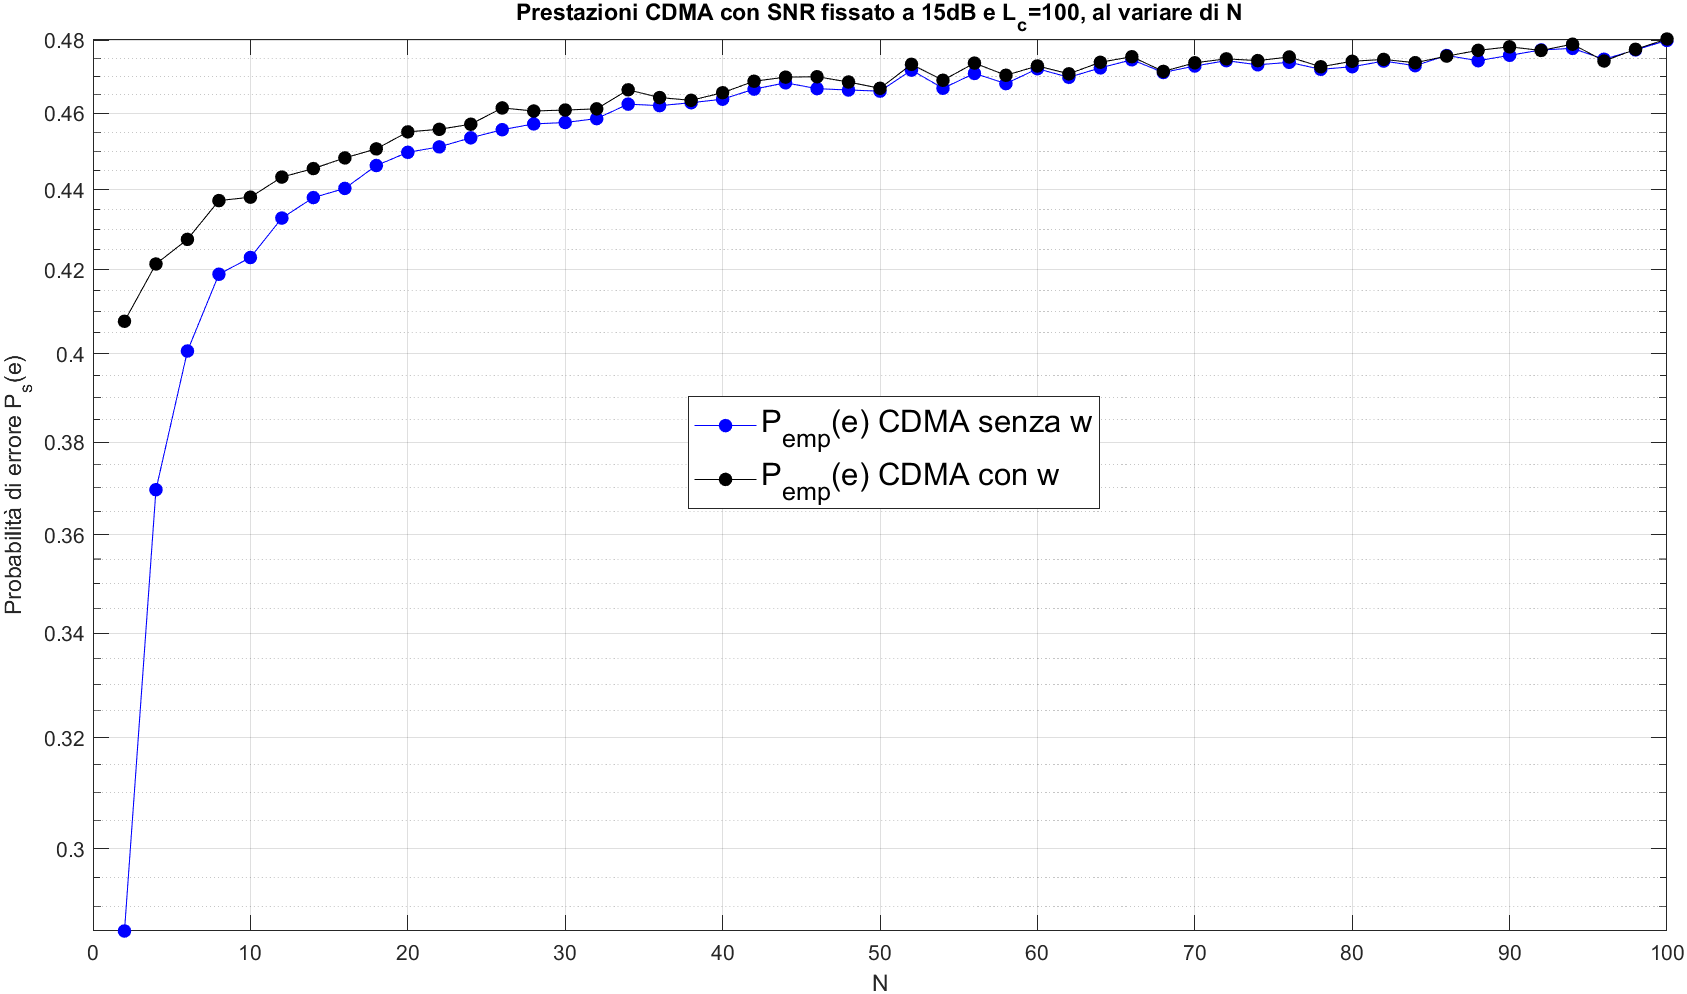
\includegraphics{images/prestazioniCDMA2.png}
\end{adjustbox}\\\\
In questa seconda simulazione è stato scelto di fissare l'\(SNR_{dB}\) a \(15\,dB\) ed \(L_c\) a \(100\) e valutare le prestazioni al variare di \(N\in[2,100]\).\vspace{.3cm}\\
Entrambe le \(P_{emp}(e)\) crescono all'aumentare di \(N\) perchè aumenta sempre più la varianza del rumore \(n\) che dipende da \(L_c\) ed \(N\), infatti \(n\sim\mathcal{N}(0,\,L_c(N-1))\).\\
Per \(N\) piccoli, quindi per \(N\in[2,30]\), si nota una maggiore differenza tra la \(P_{emp}(e)\) senza \(w\) aggiuntivo e quella con \(w\), infatti quest'ultima denota prestazioni peggiori.\\
Invece al crescere di \(N\), quindi per \(N>30\), la varianza del rumore \(n\) aumenta sempre di più per entrambe le \(P_{emp}(e)\) fino a far diventare trascurabile \(w\) rispetto ad \(n\) per la \(P_{emp}(e)\) nera, facendo sovrapporre i due grafici.